\documentclass[journal]{IEEEtran}
\usepackage{amsmath,amssymb,booktabs,graphicx,cite,url}
\usepackage[hidelinks]{hyperref}
\usepackage{tikz}
\begin{document}
\title{Does Messy Mean Wrong? Label-Sensitive Trajectory Signals Under Strengthened Coding-Agent Tests}
\author{Authors and affiliations to be confirmed\thanks{Internal draft, 13 November 2026. Not submitted or independently semantically adjudicated.}}
\maketitle
\begin{abstract}
Coding-agent runs that pass a standard benchmark can exhibit repeated terminal commands, tool errors, or unverified edits. We examine whether four frozen, low-cost trajectory indicators distinguish later failures under strengthened SWE-ABS tests. Our real-data audit matches 198 originally successful Gemini 3 Flash runs across 73 distinct SWE-bench Verified tasks to the exact submitted patch and stronger-test runner record using a joint sample, task, and patch SHA-256 key. Original runner labels are 153 PASS, 31 provisional FAIL, and 14 UNVERIFIED. A conservative documentary-reviewed primary screen retains 153 PASS and nine issue-aligned provisional FAIL runs, excludes 36, and contains only five distinct positive tasks. Duplicate terminal-command rate achieves an oriented AUROC of 0.489 (95\% task-cluster bootstrap interval 0.270--0.706); terminal-error rate achieves 0.599 (0.420--0.790). The same duplicate-command feature reaches 0.721 under a noninvalid sensitivity policy and 0.708 when all runner FAIL records are counted, demonstrating substantial label-policy sensitivity. Eight prespecified qualitative cases include high-duplication passes, low-duplication failures, questionable augmented assertions, backend skips and patch-preservation problems. These exploratory, univariate findings neither establish a reliable semantic-defect predictor nor rule out a relationship in larger samples. They instead underscore the need to report patch provenance and validity-sensitive outcome definitions when interpreting process signals.
\end{abstract}
\begin{IEEEkeywords}
Coding agents, SWE-bench, SWE-ABS, trajectory indicators, test validity, outcome sensitivity, AUROC, empirical software engineering.
\end{IEEEkeywords}

\section{Introduction}
Software-engineering agents are commonly assessed through final-patch pass/fail outcomes on benchmarks such as SWE-bench \cite{jimenez2024swebench}. Yet binary task success hides the process by which a patch was produced. AgentLens identifies differences in the quality of nominally successful trajectories \cite{sahoo2026agentlens}, while TraceProbe analyzes action sequences and notes the importance of task-dependent behavior \cite{shu2026traceprobe}. SWE-ABS adds a complementary perspective: stronger tests can reject solutions that passed an original benchmark suite \cite{yu2026sweabs}.

This motivates the question whether inexpensive observations of the \emph{original agent trajectory} help distinguish which previously successful patches survive strengthened tests. The problem is not only statistical. A runner failure may reflect an inappropriate enhanced assertion or environment; a run with skipped tests or modified agent files may be impossible to classify reliably. Therefore, treating all execution outcomes as semantic ground truth may distort an estimated association.

A preceding September draft in this project examined a synthetic six-indicator composite score and simulated outcomes. Its AUROC and logistic odds ratio were generated by an intentionally constructed synthetic relationship and \emph{are not used as results here}. The present study uses four independently defined indicators on real trajectories, exact submitted-patch matching, an explicitly provisional outcome policy, clustered uncertainty, and fixed qualitative case-selection rules.

The contribution is a reproducible, bounded study of trajectory-process association \emph{conditional on originally passing evaluation}, with careful sensitivity to stronger-test label validity. It is not a new trained detector and does not establish causal effects of agent actions.

\section{Related Work}
SWE-bench operationalizes software-maintenance tasks from GitHub issues and executable tests \cite{jimenez2024swebench}. The 500-task Verified subset underwent a separate human audit of original task and issue quality \cite{openai2024verified}; this audit is not an assessment of the newly introduced SWE-ABS assertions. SWE-ABS improves test coverage and adversarial strength and documents that pass rates are affected by enhanced evaluation \cite{yu2026sweabs}. These works motivate evaluating more than the original available tests, but the stronger suite remains an operational measurement rather than a mathematical oracle.

AgentLens assesses successful agent trajectories relative to process-quality references, detecting behaviors such as blind retries, verification omissions, and regressions \cite{sahoo2026agentlens}. TraceProbe provides trajectory-structure diagnostics and identifies cases in which process anti-patterns may primarily indicate task difficulty \cite{shu2026traceprobe}. SWE-Cycle additionally examines environment reconstruction, implementation, verification and full end-to-end issue resolution, using a hybrid execution-aware judge \cite{guan2026swecycle}. Our exact-run source pairing and documentary label sensitivity are a different, narrower target. We make no claim to be the first work on trajectory behavior or on stronger tests.

Recent community guidance stresses accurate LLM-use reporting, reproducible configuration, human evaluation when automated judgments stand in for expert assessments, and explicit limitations \cite{baltes2026guidelines}. Our technical reproduction checks meet part of that standard; the absence of independent semantic gold judgments remains a substantial gap.

\section{Research Questions}
Let one original passing run be indexed by the exact tuple $(s,t,h)$, where $s$ is sample, $t$ is SWE-bench task identifier, and $h$ is SHA-256 of the submitted UTF-8 patch. Multiple run samples can share one task and are statistically dependent.

\emph{RQ1:} Under a conservative documentary-reviewed label policy, what discrimination do four fixed trajectory indicators achieve between runner PASS and issue-aligned provisional FAIL, measured by oriented univariate AUROC?

\emph{RQ2:} How does discrimination change when the prespecified alternative policies include broader runner failures or hypothetically treat coverage-limited cases as PASS?

\emph{RQ3:} What do prespecified positive, negative, contradictory, and validity-challenge cases reveal about the interpretation of a process indicator and a stronger-test outcome?

None of these research questions asks for a calibrated risk score, held-out prospective prediction or causal effect.

\section{Data and Outcome Measurement}
\subsection{Exact original-patch matching}
The source is the public Gemini 3 Flash agent-trajectory dataset. The exact Hugging Face dataset identifier and pinned revision are recorded in the replication repository\footnote{\url{https://github.com/Foysal-Munsy/sweabs-free-eval}}. The pinned source snapshot has 296 rows, of which the evaluated population contains 198 originally resolved runs (63, 68 and 67 from samples 1, 2 and 3), spanning 73 distinct tasks. Each original trace has ordered messages and function tool calls, a complete submitted patch and a sample/task identifier.

We accept a source row only on exact \texttt{(sample, instance\_id, SHA256(patch))} agreement with the evaluation manifest. The extraction code rejects absent, mismatched, or duplicate identity keys instead of taking a different model patch on the same task. All 198 runs are exact-matched. This does not establish that all issues or agents were randomly sampled.

\subsection{Stronger-test execution and audit}
The strengthened-test source is the SWE-ABS verified-task augmented-test dataset, at the precise revision frozen in the public replication manifest. GitHub Actions served as the Docker-capable evaluation runner; original per-patch tests and raw evidence, not the green workflow status alone, determine provisional outcomes. An 83-record historical and a 115-record subsequent audit produced the immutable runner v2: 153 PASS, 31 provisional FAIL and 14 UNVERIFIED.

Nine UNVERIFIED runs had backend-dependent skipped augmented tests, four had original patch/test file overlap, and one lacked sufficient tested-tree integrity evidence. Independent, separately versioned later controlled tests improve evidence but do not overwrite the old runner record. Under the original 31 runner failures, documentary issue/merged-PR review marked nine \texttt{valid\_failure}, four \texttt{invalid\_test}, two \texttt{environment\_sensitive} and 16 \texttt{unresolved}. The review was AI-assisted, not a human/maintainer semantic truth oracle.

\begin{table}[t]
\centering
\caption{Frozen provisional outcome policies (run-level counts).}
\label{tab:labels}
\begin{tabular}{lrrr}
\toprule
Policy & PASS (0) & FAIL (1) & Excluded\\
\midrule
Primary reviewed &153&9&36\\
Noninvalid sensitivity &153&27&18\\
All runner FAIL &153&31&14\\
Skipped-as-PASS scenario &162&9&27\\
\bottomrule
\end{tabular}
\end{table}

The primary 162 eligible rows cover 61 tasks but only \emph{five} distinct positive tasks; multiple positive samples from the same issue do not create independent evidence. All 153 original PASS records are \emph{runner-observed} PASS, not fully adjudicated semantic correctness.

\section{Outcome-Validity Audit and Cohort Dependence}\label{sec:auditing}
\subsection{Sampling and classification transparency}
Table~\ref{tab:cohort} separates distinct agent runs from distinct tasks. All 198 selected trajectories had a recorded original benchmark success, yet their strengthened-test outcomes remained provisional and could not all be safely assigned to a binary target. A simple binary conversion of the 14 UNVERIFIED rows would introduce extra assumptions that the historical runner did not verify.

\begin{table}[t]
\caption{Original strengthened-test attempt counts. Different samples may share a task identifier.}
\label{tab:cohort}
\centering
\begin{tabular}{lrrrr}
\toprule
Source sample & Runs & PASS & FAIL & UNVERIFIED\\
\midrule
1 & 63 & 48 & 10 & 5\\
2 & 68 & 53 & 11 & 4\\
3 & 67 & 52 & 10 & 5\\
\midrule
Total &198 &153 &31 &14\\
\bottomrule
\end{tabular}
\end{table}

Historical runner records and the agent patch form a \emph{measurement chain}: the original passing agent trajectory provides the submitted patch; that patch must survive baseline checkout and augmented-test installation; the relevant tests must execute; their assertions must be defensible relative to the task; and tool or CI success must not be confused with task success. These gates are conceptually distinct. Passing the first gates does not guarantee the last.

\subsection{Why 31 runner failures are not 31 gold positives}
The 31 runner FAIL rows include nine review-supported issue-aligned cases, four enhanced-test assertions classified as invalid, two Python/runtime-sensitive cases, and 16 whose issue-level semantic validity could not be resolved from available documentary evidence. Even the nine supported cases are \emph{provisional}: the categorization was AI-assisted issue/PR/test review, not independent human or maintainer adjudication.

\begin{table}[t]
\caption{Documentary review of 31 original runner FAIL records. These are not independent semantic gold labels.}
\label{tab:reviewdispositions}
\centering
\begin{tabular}{lr}
\toprule
Review status & Runner FAIL runs\\
\midrule
Issue-aligned (review-supported) &9\\
Invalid augmented assertion &4\\
Environment-sensitive contract &2\\
Unresolved issue-level validity &16\\
\bottomrule
\end{tabular}
\end{table}

The nine positive records in the conservative analysis arise from only \emph{five} task identifiers. A task-cluster bootstrap protects against treating all runs as independent, but it cannot turn five positive task families into a well-powered set of independent defect mechanisms. The cohort is also selected conditional on original PASS: it does not represent all coding-agent attempts.

\subsection{Three distinct objects of inference}
An \emph{execution result} describes a suite and environment. A \emph{documentary review category} describes available issue/test reasoning. A \emph{semantic defect label} would require a validated contract and independent assessment. This study has the first two in versioned form, but not the third. The missing third object is a scientific limitation, not a formatting issue.


\section{Frozen Process Indicators}
The four indicators were specified on 12 November 2026 before all-run feature extraction and the inspection of feature--outcome associations. This is a project-stage freeze, \emph{not} a claim of prospective preregistration before all prior outcome inspection. Terminal commands are normalized by collapsing whitespace and retaining letter case.

\begin{align}
d &= \frac{\text{terminal calls repeating an earlier exact command}}
              {\max(1,\text{terminal calls})},\\
e &= \frac{\text{matched explicit nonzero/error terminal replies}}
              {\max(1,\text{terminal calls})},\\
v &= -\mathbb{1}[\text{any regex-recognized test invocation}],\\
p &= \text{editor calls after last recognized test invocation}.
\end{align}
These are independently scored in the original direction, with higher values indicating \emph{presumed} messiness. For $d$, duplicates can occur at any separation, not merely adjacent repetitions. For $e$, unique tool-call IDs and explicit exit/error flags are required; missing replies do not count as zero errors. Verification recognizes a fixed regex including \texttt{pytest}, \texttt{unittest}, \texttt{runtests.py}, \texttt{tox} and \texttt{nosetests} commands; arbitrary scripts and other activities are not broadly counted. The count $p$ is missing if no command matches this rule. In 198 exact-run feature rows, 191 contain recognized verification; the seven remaining do not necessarily lack all real verification.

The features measure observable tool events, not whether an agent understood the code or whether a test was sufficient. The six-feature synthetic composite score from the superseded draft is not fitted, transplanted, or interpreted in this real-data analysis.

\section{Statistical Analysis}
For one fixed score $z$, the oriented area under the receiver operating characteristic curve is
\begin{equation}
\mathrm{AUROC}=\Pr(z^+>z^-)+\tfrac12\Pr(z^+=z^-),
\end{equation}
evaluated over positive--negative \emph{run} pairs. The feature direction is frozen, never reversed to report a higher AUROC. A value of 0.5 corresponds to chance-level pairwise ranking \emph{for that operational target}, not calibrated deployment performance.

Uncertainty uses 500 task-identifier-cluster bootstrap resamples (seed 20261112), retaining all runs belonging to a sampled task. The corrected, independently checked v2 implementation fixes an archived v1 bootstrap index-scaling problem. Only 496 of 500 primary resamples contain both classes. Resampling does not eliminate label error, selective original PASS enrollment, or unmeasured task difficulty. Four indicators and four targets were analyzed without model training, feature weighting, threshold tuning, or external test data. Exploratory Step 11 task-macro, within-project, trajectory-length and leave-one-positive-task-out checks are post-hoc and are not promoted to confirmatory findings.

\section{Quantitative Results}
\begin{table}[t]
\centering
\caption{Conservative primary AUROC with 95\% task-cluster bootstrap CI.}
\label{tab:primary}
\begin{tabular}{lccc}
\toprule
Indicator & $n$ & AUROC & CI\\
\midrule
Duplicate command rate &162&0.489&[0.270, 0.706]\\
Terminal error rate &162&0.599&[0.420, 0.790]\\
No recognized verification &162&0.480&[0.459, 0.497]\\
Editor after verification &156&0.435&[0.166, 0.757]\\
\bottomrule
\end{tabular}
\end{table}

The conservative duplicate-terminal rate AUROC is $0.489$ (95\% task-cluster interval $0.270$--$0.706$), consistent with weak or inconclusive ranking. The terminal-error rate is $0.599$ ($0.420$--$0.790$). No indicator establishes robust discrimination with this small cluster-positive sample. The near-constant verification indicator should not be mistaken for well-powered evidence of an exact null.

\begin{table}[t]
\centering
\caption{Frozen indicators under four different provisional targets.}
\label{tab:sens}
\resizebox{\columnwidth}{!}{%
\begin{tabular}{lcccc}
\toprule
Target & Duplicate & Error & No verify & Late edit\\
\midrule
Primary &0.489&0.599&0.480&0.435\\
Noninvalid &0.721&0.498&0.499&0.405\\
Runner-only &0.708&0.477&0.497&0.398\\
Skipped-as-PASS &0.478&0.588&0.481&0.448\\
\bottomrule
\end{tabular}}
\end{table}

The same duplicate-command score has AUROC $0.721$ (CI $0.565$--$0.857$) when the reviewed \texttt{invalid\_test} records are excluded but unresolved and environment-sensitive runner failures are retained, and $0.708$ ($0.562$--$0.834$) when all runner FAILs are included. A hypothetical skipped-as-PASS analysis has AUROC $0.478$ ($0.255$--$0.686$). These are meaningfully different \emph{label policies}, not competing estimates of independently established true bug prevalence. None supports a calibrated or externally generalizable early-warning classifier.

\section{Task-Aware Robustness and Sensitivity Visualization}\label{sec:robust}
Figure~\ref{fig:labelpolicy} makes target-definition dependence explicit. Each interval is a bootstrap confidence interval \emph{for a different analysis population}, not a paired estimator comparison on identical cases. The original score and direction are held fixed. The primary duplicate-rate interval includes chance ranking; the broader runner intervals do not. This indicates label-selection sensitivity, not validated semantic-defect classification.

\begin{figure}[t]
\centering
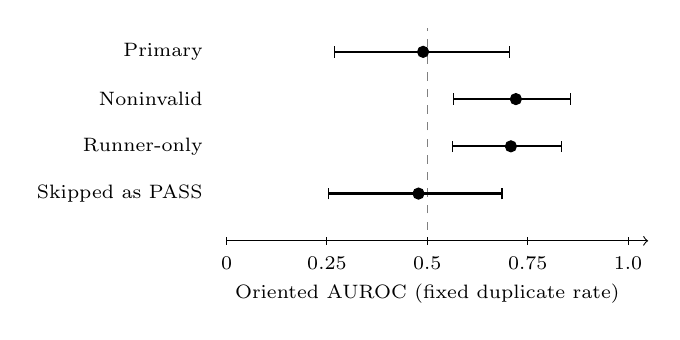
\begin{tikzpicture}[x=5.1cm,y=0.60cm, font=\scriptsize]
\draw[->] (0,0)--(1.05,0);
\foreach \x in {0,0.25,0.5,0.75,1.0} {
  \draw (\x,-0.08)--(\x,0.08);
  \node[anchor=north] at (\x,-0.13) {\x};
}
\draw[dashed,gray] (0.5,0.23)--(0.5,4.5);
\node[anchor=east] at (-0.035,4) {Primary};
\node[anchor=east] at (-0.035,3) {Noninvalid};
\node[anchor=east] at (-0.035,2) {Runner-only};
\node[anchor=east] at (-0.035,1) {Skipped as PASS};
\foreach \lo/\hi/\point/\y in {
  0.269582/0.705747/0.489470/4,
  0.565309/0.856875/0.720528/3,
  0.562218/0.834433/0.708096/2,
  0.254538/0.685949/0.478052/1
}{
  \draw[thick] (\lo,\y)--(\hi,\y);
  \draw (\lo,\y-0.12)--(\lo,\y+0.12);
  \draw (\hi,\y-0.12)--(\hi,\y+0.12);
  \filldraw (\point,\y) circle (2pt);
}
\node[anchor=north] at (0.5,-0.70) {Oriented AUROC (fixed duplicate rate)};
\end{tikzpicture}
\caption{Duplicate-terminal-rate AUROC (point) and task-cluster bootstrap 95\% confidence interval (whiskers) under four frozen but different label policies. Dashed line denotes 0.5. Inputs: corrected Step 10 v2.}
\label{fig:labelpolicy}
\end{figure}

Step 11 robustness checks were computed \emph{after} the main AUROCs had been seen. They are therefore exploratory interpretation stress tests, not confirmatory improvements to the frozen methodology. Table~\ref{tab:robustness} shows how weighting and restricting comparable units changes the duplicate rate's score.

\begin{table}[t]
\caption{Exploratory duplicate-rate robustness under distinct analysis units; not held-out prediction.}
\label{tab:robustness}
\centering
\resizebox{\columnwidth}{!}{%
\begin{tabular}{lcc}
\toprule
Descriptive analysis & Primary & Runner-only\\
\midrule
Run-level AUROC &0.489&0.708\\
Task-macro AUROC$^\dagger$ &0.522&0.741\\
Within-project AUROC$^\ddagger$ &0.390&0.738\\
Leave-one-positive-task-out range &0.382--0.620&0.683--0.759\\
Positive task IDs &5&15\\
\bottomrule
\end{tabular}}
\vspace{1mm}

{\footnotesize $^\dagger$Unanimously labeled tasks only; discordant tasks excluded. $^\ddagger$Pairs from different tasks in the same project. Neither method measures accuracy on previously unseen tasks.}
\end{table}

For the primary target, task-macro AUROC is 0.522, within-project AUROC is 0.390, and removing each positive task family gives run-level estimates from 0.382 to 0.620. Which task appears in the primary positive set therefore matters greatly. For the runner-only sensitivity, the corresponding leave-one-positive-task-out range is 0.683 to 0.759 across 15 distinct positive tasks; this does not prove those broader positives are true semantic defects.

An explicitly post-hoc trajectory-length comparator also yielded AUROC 0.660 under the primary policy, while duplicate rate versus step count had Spearman correlation $-0.112$. These descriptive checks were not selected or calibrated before outcomes and therefore cannot be interpreted as a new validated predictor. Task-difficulty confounding has not been eliminated. All exploratory inputs are versioned in the public Step 11 robustness JSON.


\section{Prespecified Qualitative Case Studies}
The Step 12 selection rule was committed before inspection of individual selected cases. The first four slots deterministically chose the highest and lowest duplicate-command-rate primary PASS and FAIL examples while excluding already chosen task identifiers; four further slots selected invalid-test, environment, skip and patch-overlap challenges. All eight identities were checked against the exact patch hashes. GitHub Actions independently recounted eight raw source traces and 112 indicator values with zero mismatches. The cases are \emph{outcome-ranked illustrative extremes}, not a representative sample.

Among reviewed FAILs, SymPy issue 15599 sample 1 had 12 repeated commands among 42 terminal calls (0.286) and failed issue-aligned augmented \texttt{Mod} tests; broader mathematical assertions were not independently human-adjudicated. Django issue 14311 sample 2 had only 1/46 repeats (0.022), yet the stronger runner failed two tests on module-reload behavior and recorded 16 explicit terminal error observations. The low duplicate-rate FAIL is a contradiction to the claim that frequent exact repetition is necessary for failure.

Django issue 13820 sample 1 had 10/25 repeated commands (0.400), including ten adjacent repetitions, but passed 4/4 executed enhanced tests. This is not proof of full semantic correctness, just a high-duplication \emph{runner PASS}. Django issue 11333 sample 3 had 0/19 repeats and passed all eight enhanced tests, despite two explicit terminal error observations. Together the cases show that repeated commands and observed runner outcomes do not form a deterministic relationship.

In the four challenge slots, Django issue 11848 failed an RFC850 year-wrap assertion that documentary review assessed as inconsistent with the cited protocol; issue 15916 involved Python-version-sensitive \texttt{staticmethod} callable behavior; issue 12039 originally skipped four database tests and remained UNVERIFIED even though a separate PostgreSQL rerun later passed 13 added tests; and issue 11206 had model/test-file overlap in the original runner, with a separate patch-preserving merge reproducing five disputed signed-zero assertions. These examples separate execution evidence from issue-appropriate semantic correctness.

\section{Discussion}
\subsection{Supported interpretation}
The evidence supports exact trace-to-patch matching and reproducible univariate association measurement, while showing that a previously successful agent's apparent stronger-test label can be conditional on the enhanced assertion, backend and patch-preservation boundary. The conservative primary effect is negative or inconclusive and the broader runner-only effects depend on accepting less-validated failures. Choosing the most flattering AUROC would change the question.

\subsection{Competing explanations}
Task difficulty may jointly increase repeated commands and stronger-test failure risk. Identical commands can be appropriate repeated verification. Tool errors may stem from setup failures. Some strengthened expectations can exceed issue requirements, while original PASS-only selection can induce collider bias. Task-aware uncertainty addresses dependence across repeated task samples, not these causal, selection or validity threats. We cannot decide among these explanations from the current data.

\subsection{Implications}
A practical process-warning signal would require independent semantic labels, more distinct positive tasks, task-disjoint replication on other agents, then prospective thresholds, precision--recall and calibration where relevant. These are proposed extensions, not experiments silently added after observing our results. A credible alternative scientific takeaway is that code-agent evaluation needs careful \emph{oracle auditing} alongside process diagnostics, even when the underlying predictive association is weak.

\section{Interpretive Boundaries and Future Validation}\label{sec:interp}
\subsection{Why the target determines the conclusion}
The conservative analysis attempts to avoid treating a disputed augmented assertion as a true defect. The broader runner-only analysis instead asks whether an original process measure ranks \emph{whatever the existing runner reports as failure}. Either may be relevant to a different operational goal, but they are not interchangeable. For true \emph{semantic correctness}, neither label policy supplies a fully validated reference standard.

This distinction is not unique to the present study. SWE-bench Verified was introduced as a human-filtered subset of the original benchmark \cite{openai2024verified}; later commentary raised concerns about training-data exposure and benchmark task/test design \cite{openai2026benchmark}. This external critique does \emph{not} establish contamination of the Gemini 3 Flash source studied here; no sample-specific contamination test was conducted. SWE-Cycle evaluates environment setup, code generation and verification together, and proposes hybrid execution-aware judgments \cite{guan2026swecycle}. Such designs provide competing alternatives to relying on one runner outcome.

\subsection{Proposed independent semantic annotation extension}
A high-priority extension would independently assess the issue-level relevance of the 31 historical runner FAILs and relevant coverage-limited records. To prevent confirmation bias, experts should receive the original issue, exact model patch, pinned augmented-test diff, base environment and observed test output \emph{without seeing the trajectory score or desired study result}. At least two experienced engineers would independently record one of four categories per disputed assertion: (i) issue-required semantic defect; (ii) unsupported or wrong augmented assertion; (iii) environment/harness-confounded; (iv) unresolved from available evidence. An adjudicator could resolve disagreements without rewriting the frozen historical results.

Reviewer agreements, rubric versions and unresolved cases would be archived separately. A future analysis could then compare documentary labels with expert judgments, add distinct positive tasks, and repeat the study on another agent/model. This paragraph is a \emph{prospective proposal}, not a report of completed human validation.

\subsection{Why not report a calibrated detector today?}
The earlier synthetic paper used logistic regression and a six-feature composite with simulated outcomes. Neither has been re-fitted on real runs. The current five positive task families cannot justify stable deployment thresholds, externally assessed probability calibration or causal conclusions. PR-AUC and decision curves would become meaningful for a future deployment-oriented question only after label adjudication, adequate distinct positive tasks and a genuine holdout design. Their absence is a limitation for practical prediction, not a result that should be invented to satisfy an old synthetic-study reviewer checklist.

\subsection{Negative findings are not proof of independence}
The results do not prove that clean process and correct patches are unrelated. They show that four particular inexpensive process proxies fail to show robust discrimination under one small, conservative runner-association target, and that alternate target definitions shift the ranking substantially. Different populations, other process metrics or better semantic oracles could yield other results. Conversely, even an impressive runner-only AUROC would not establish semantic correctness or causality.


\section{Threats to Validity}
\textbf{Outcome validity:} Only nine of 31 provisional runner FAILs have documentary support; no expert human gold labels exist for the 31, and all 153 runner PASS labels remain test-limited. Fourteen historical UNVERIFIED outcomes are unchanged by new separate-runtime checks. A green CI run is not an agent-level PASS.

\textbf{Construct validity:} Four regex/count proxies cannot capture reasoning intent, actual test sufficiency, or whether a repeated command was rational. No six-indicator synthetic score is presented as real evidence.

\textbf{Internal and statistical validity:} Only five distinct primary positive tasks, 61 total primary task IDs, multiple run samples per task, observational process measures, and possible task-difficulty confounding sharply limit the inferential strength of AUROC/bootstrap intervals. The primary point estimate near 0.5 is not proof of no effect.

\textbf{Selection/external validity:} The cohort consists solely of originally successful Gemini 3 Flash runs from a bounded public corpus. Its behavior may differ from failed original runs, different agents, repositories, models and deployment conditions.

\textbf{Reproducibility:} Public derived artifacts, pinned source revision, exact patch hashes, scripts and CI provenance are provided, but the original Docker-tested trees and privately held result ZIPs are not wholly republished; subsequent PostgreSQL and patch-preserving executions are not identical historical runs.

\textbf{AI-assisted research and manuscript preparation:} AI-assisted documentary review and ChatGPT GPT-6-assisted manuscript drafting do not replace independent expert evaluation. Human authors must verify the final scientific content, bibliography, originality, author list and venue-specific required disclosures before submission \cite{baltes2026guidelines}.

\section{Artifact Availability and Research Disclosure}\label{sec:replication}
\subsection{Public reproduction boundary}
The public replication repository \url{https://github.com/Foysal-Munsy/sweabs-free-eval} contains exact run identifiers, frozen feature definitions, source-aligned feature extraction code, the immutable original 198-run runner ledger, conservative and sensitivity label manifests, corrected bootstrap analysis, selected case definitions, and read-only GitHub Actions workflows. Original trajectory and strengthened-test datasets are available at the pinned revisions specified in that manifest. Raw historical per-patch ZIP files are privately archived and some CI artifacts are short-lived. Public derived-output and pinned-source gates can be reproduced, but they do not provide identical access to every historical Docker-tested tree.

\subsection{Software checks versus semantic adjudication}
Independent Step 9 reproduction matched 198/198 exact original runs and the archived derived features. Step 12 independently recounted eight frozen source trajectories and checked 112 feature values with zero mismatches. Step 10 corrected bootstrap output was also independently recomputed and verified. A separate LaTeX build creates a PDF from the version-controlled source. These checks support measurement and computation \emph{reproducibility}; none establishes independent expert agreement on enhanced-test semantic validity.

\subsection{AI assistance and accountability}
AI assistance was used in the documentary review of questionable enhanced assertions. ChatGPT GPT-6 was subsequently used to organize checked source evidence, draft LaTeX prose and tables, and prepare this manuscript. These uses do not replace human expert adjudication or researcher responsibility. The responsible author team must confirm the exact AI systems and roles, final bibliography, author contributions and journal-specific disclosures before submission. Empirical LLM-SE guidance emphasizes declaring model roles, source configurations, reproducibility limitations and validation against appropriate human reference judgments \cite{baltes2026guidelines}. The present paragraph is a draft disclosure pending author sign-off.


\section{Conclusion}
We analyzed four prespecified trajectory indicators against strengthened-test runner outcomes for 198 originally successful coding-agent runs. Conservative reviewed positive labels yield duplicate-command AUROC $0.489$ with wide task-cluster uncertainty; broader runner-outcome policies yield $0.708$--$0.721$ for the unchanged same indicator. The evidence therefore does not establish a robust semantic-defect predictor, but does establish substantial sensitivity to provisional label policy. Eight exact-patch cases identify contradictions and validity challenges behind this quantitative difference. Future research needs independent semantic adjudication and stronger task/model replication before using process cleanliness as a reliable substitute for tested correctness.

\bibliographystyle{IEEEtran}
\bibliography{references}
\end{document}
